\section{Simulation Analysis}
\label{sec:simulation}

In this section, we can find the results of the topics required in the simulation analysis. The numeric results or graphics are presented alongside a short explanation of the interpretation of the problem. All of the results were obtained using NGSpice and the section is divided in three different subsections. 

\subsection{Output Voltage Gain}

\begin{figure}[H]\centering
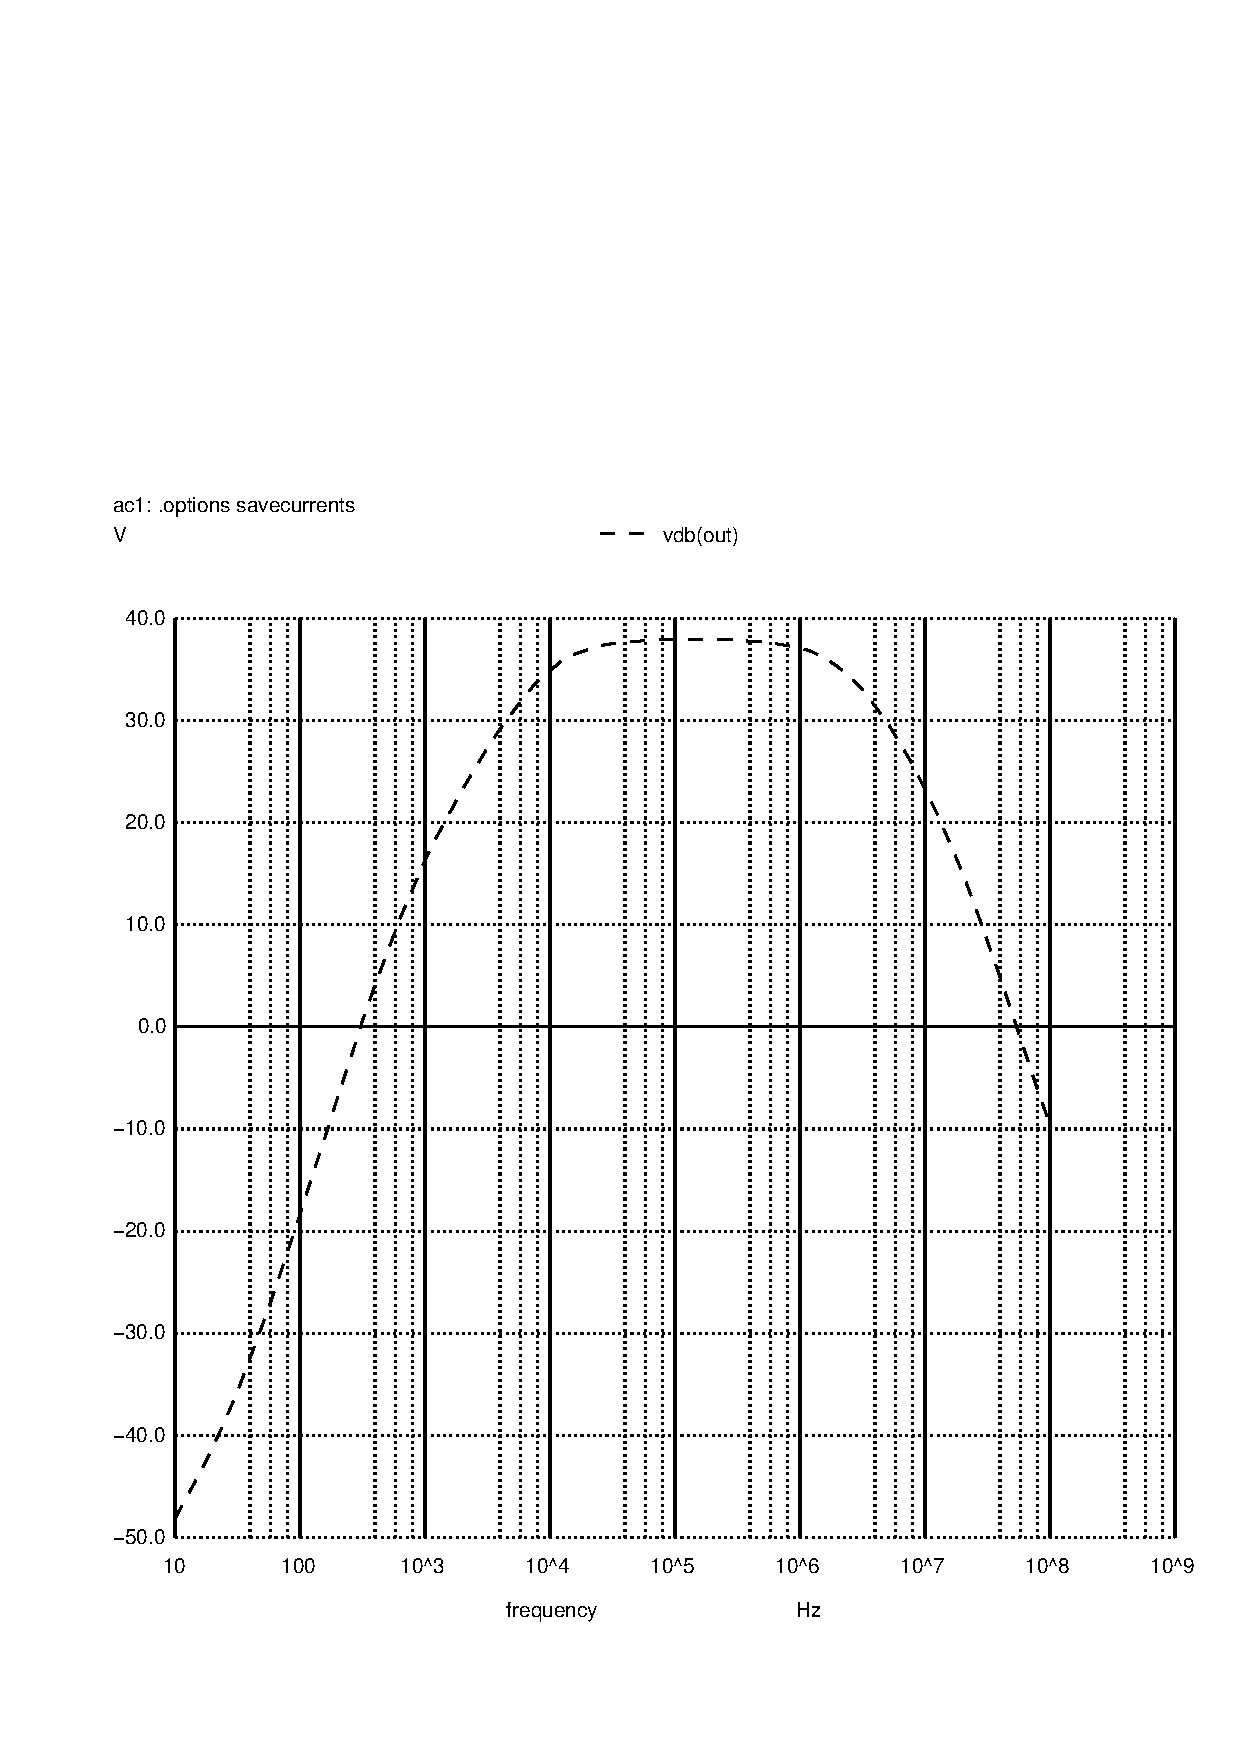
\includegraphics[trim= 0cm 0cm 0cm 10cm, clip, width=0.7\textwidth]{vo2f.pdf}
\caption{The Output Voltage of the Output Stage of a Common Collector Amplifier.}
\label{fig:sim_output}
\end{figure}

where $f$ is expressed in Hertz (Hz) along the x-axis\\
and $v_{dB_{out}}$, the output voltage of the amplifier, is expressed in  in Volts (V) using a decibel scale along y-axis.

\begin{table}[H] \centering
  \begin{tabular}{|l|r|}
    \hline    
    {\bf NGSpice Formula} & {\bf Output Voltage Gain (V)} \\ \hline
    \input{outvoltagegain_TAB}
  \end{tabular}
 \label{tab:outvoltagegain}
\end{table}

\subsection{Bandwidth and Cut-Off Frequencies}

\begin{table}[H] \centering
  \begin{tabular}{|l|r|}
    \hline    
    {\bf Variable} & {\bf Frequency Value (Hz)} \\ \hline
    \input{cutofffreq_TAB}
  \end{tabular}
 \label{tab:cutofffreq}
\end{table}

where $f_1$ is the lower cut-off frequency,\\
a$f_1$ is the upper cut-off frequency and\\
$f_2-f_1$ is the bandwith (the difference between the upper and lower cut-off frequencies).

\subsection{Input and Output Impedances}

\begin{table}[H] \centering
  \begin{tabular}{|l|r|}
    \hline    
    {\bf NGSpice Formula} & {\bf Input Impedance Value ($\Omega$): $a,b$ from $Z_{in}=a+bj$}\\ \hline
    \input{inputimp_TAB}
  \end{tabular}
 \label{tab:inputimp}
\end{table}

\begin{table}[H] \centering
  \begin{tabular}{|l|r|}
    \hline    
    {\bf NGSpice Formula} & {\bf Output Impedance Value ($\Omega$)}\\ \hline
    \input{outimpedance_TAB}
  \end{tabular}
 \label{tab:inputimp}
\end{table}
